Alles wat je op de prompt intypt wordt opgevangen door de shell. De shell is een schil rond de kernel die commando's van
gebruikers aanneemt en deze doorgeeft naar de kernel. Shell is het Engelse woord voor schelp en een schelp zorgt ervoor
dat het weekdier dat in de schelp leeft beschermt wordt tegen de buitenwereld. Dat is bij de shell net zo, de shell
beschermt de kernel tegen de gebruiker. De shell wordt ook wel een command interpreter genoemt omdat hij commando's van
de gebruiker interpreteert.

Linux gebruikt standaard de bash shell. Bijna elke linux distributie levert deze mee en heeft deze als standaard shell.
Van oudsher werd op Unix systemen sh meegeleverd. Het was een van de eerste programma's die werd geschreven voor Unix
door Ken Thompson. Tussen 1976 en 1979 schreef Stephen Bourne een vervanging voor sh wat de standaard werd in Version 7
Unix. De naam bleef echter sh op het Unix systeem. Toen het GNU project een vrij en open source systeem wilde maken was
ook daar een van de eerste programma's die er moest komen een shell. Dat werd bash, de naam bash staat voor Bourne
Again SHell. Het is een open source versie van de shell geschreven door Stephen Bourne.

Unix en Linux commando's en bestandsnamen zijn case sensitive. Dat betekent dat `hello.txt' niet hetzelfde is als
`Hello.txt'. Dit zijn twee verschillende bestanden.

Commando's of opdrachten aan de shell hebben een vaste vorm (syntax). Ze zien er zo uit:

\begin{lstlisting}[language=bash]
commando<spatie>optie(s)<spatie>argument(en)
\end{lstlisting}

De spaties zorgen ervoor dat de shell weet wanneer een volgend deel begint, voor de eerste spatie staat het commando,
daarna volgen er geen of enkele opties en tot slot zijn er geen of enkele argumenten. Bijna alle commando's houden deze
syntax aan, hoewel er ook uitzonderingen zijn.

Het commando ls laat een lijst met bestanden zien. Als we het gebruiken zonder argumenten dan ziet dat er ongeveer uit als in figuur \ref{fig:lsDir}
\begin{figure}[h]
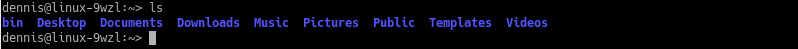
\includegraphics[width=0.9\linewidth]{linuxreader-img023.png}
\label{fig:lsDir}
	\caption{Directory listing}
\end{figure}

Opties worden van argumenten onderscheiden doordat opties beginnen met een min-teken (-). Geven we aan ls een optie me,
bijvoorbeeld -r voor reverse, of wel sorteer omgekeerd dan zien we wat we in figuur \ref{fig:lsRevDir} zien.
\begin{figure}
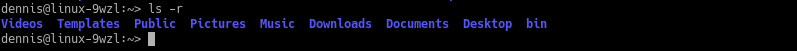
\includegraphics[width=0.9\linewidth]{linuxreader-img024.png}
	\label{fig:lsRevDir}
	\caption{Reverse order listing}
\end{figure}
We zien nu dat Videos vooraan staat en bin achteraan.

We kunnen ook meerdere opties meegeven. De optie -l geeft een long
list, ofwel een lijst die veel meer informatie per bestand of directory laat zien.
\begin{figure}[h]
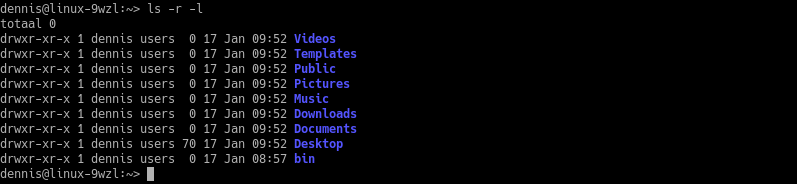
\includegraphics[width=0.9\linewidth]{linuxreader-img025.png}
	\label{fig:lslDir}
	\caption{Reverse and long listing}
\end{figure}
Je mag de opties apart meegeven
zoals we in figuur \ref{fig:lslDir} gedaan hebben maar je mag ze ook samenvoegen zoals:

\begin{lstlisting}[language=bash]
$ ls -lr
\end{lstlisting}
of
\begin{lstlisting}[language=bash]
$ ls -rl
\end{lstlisting}

We kunnen ook een argument meegeven, bijvoorbeeld:
\begin{lstlisting}[language=bash]
$ ls Documents/
\end{lstlisting}
Het argument is de naam van een directory, in dit geval Documents, en we krijgen geen output omdat de directory leeg
is.

De linux shell heeft ook een handigheidje om het leven makkelijker te maken, of beter om minder te hoeven typen, dat
handigheidje heet automatisch aanvullen. Als je op de prompt een p typt zonder een enter te geven en daarna de
tab-toetst indrukt dan gebeurd er niets, druk je nog een keer op de tab-toets dan krijg je de melding:

\begin{lstlisting}[language=bash]
Display all 177 possibilities (y or n)
\end{lstlisting}

Type n want we willen niet 177 mogelijkheden zien. Wat het systeem ons verteld heeft is dat het 177 commando's kent die
met een p beginnen, voegen we nu aan onze p een w toe en typen we 1x tab. Dan vult de shell dit aan met de d en staat
er pwd.

Dit automatische aanvullen kun je doen met commando's maar ook met bestanden en directories. Er wordt weleens gezegd dat
je het toetsenbord van een Linux-beheerder kan herkennen aan de versleten tab-toets.

